\documentclass[a4paper, 12pt]{article}
% \documentclass{report}
% \usepackage{geometry}
% \geometry{
%  a4paper,
%  total={170mm,257mm},
%  left=20mm,
%  top=20mm,
%  }
%% Language and font encodings
\usepackage[english]{babel}
\usepackage[utf8x]{inputenc}

\usepackage{booktabs}
\usepackage{tabu}
\usepackage[T1]{fontenc}

%% Sets page size and margins
\usepackage[a4paper,top=2cm,bottom=2cm,left=2cm,right=2cm]{geometry}

%% packages
\usepackage{graphicx}
\usepackage{caption}
\usepackage{subcaption}
\usepackage{cite}
%\usepackage[backend=biber,style=verbose]{biblatex}
\usepackage{amsmath,amssymb,amsfonts}
\usepackage{algorithm}
\usepackage{forloop}
\usepackage{listings}
\usepackage{algpseudocode}
% \usepackage{textcomp}
\usepackage{wasysym}
\usepackage{xcolor}
\usepackage[colorinlistoftodos]{todonotes}
\usepackage[colorlinks=true, allcolors=blue]{hyperref}
\usepackage{soul}

\setlength{\marginparwidth}{2cm}

% Allow subsubsubsection as a sectioning level
\usepackage{titlesec}

\titleclass{\subsubsubsection}{straight}[\subsubsection]
\newcounter{subsubsubsection}[subsubsection]
\renewcommand\thesubsubsubsection{\thesubsubsection.\arabic{subsubsubsection}}

\titleformat{\subsubsubsection}
  {\normalfont\normalsize\bfseries}{\thesubsubsubsection}{1em}{}
\titlespacing*{\subsubsubsection}
  {0pt}{3.25ex plus 1ex minus .2ex}{1.5ex plus .2ex}

% ---- Numbering depth ----
\setcounter{secnumdepth}{4}

% ---- ToC formatting ----
\usepackage{tocloft}

% ---- ToC formatting for subsubsubsection ----
\makeatletter
\newcommand{\l@subsubsubsection}{\@dottedtocline{4}{7em}{4em}}
\makeatother

% Show numbering & ToC down to subsubsubsection
\setcounter{tocdepth}{4}

% ---------------------------------------

\usepackage{booktabs}
\usepackage{tabularx}
\usepackage{multirow}
\usepackage{array}
\usepackage{enumitem}
\newcolumntype{Y}{>{\raggedright\arraybackslash}X}
\setlist[itemize]{leftmargin=*,topsep=1pt,itemsep=1pt,parsep=0pt}

\begin{document}
\begin{titlepage}
		%\pagecolor{pink}
		%\maketitle
		\begin{center}
			
			\Large
			
			\textbf{UNIVERSITY OF MORATUWA}
			
			\vfill
			\large
			Faculty of Engineering \\
			\vfill
			
\includegraphics[height=50mm]{images/University_of_Moratuwa_logo.png}
			\vfill
			Registered Module No: CS4203 \\

			\vfill
            \textbf{Advancing Scalability Approaches in Blockchain Systems}\\
            \medskip
			Project Proposal \\
			
			\vfill
			\textbf{Date of Submission:} \\
			\medskip
			\today \\

            \vfill
            \textbf{Team Members:} \\
			\medskip
			Perera M.V.D.P.D.S: 200012D \\
            Gamage M.S: 200652D  \\
            Harshana Lakshara : 200189M\\
            Lishan Fernando : 200012G

            \vfill
            \textbf{Supervisors:} \\
			\medskip
            Dr. Sunimal Rathnayake (University of Moratuwa)  \\
          
			
			
			\vfill
			\textbf{Department of:}  \\
			\medskip
			Computer Science and Engineering\\
		\end{center}
	\end{titlepage}

\date{}
\tableofcontents
\newpage


\section{Introduction}
\lstdefinestyle{yamlStyle}{
  language=YAML,
  basicstyle=\ttfamily,
  keywordstyle=\color{blue},
  commentstyle=\color{gray},
  stringstyle=\color{green},
  morecomment=[l]{\#},
  morekeywords={example, key, value}
}

\vspace{12pt}

Blockchain technology has emerged as a transformative innovation, attracting attention from academia, industry, and governments alike. It provides a secure, distributed ledger that enables trust among untrusted entities without relying on centralized authorities or intermediaries. Its defining properties including immutability, transparency, auditability, autonomy, and resilience position blockchain as one of the most disruptive digital technologies of the past decade \cite{sanka2021systematic}.

\vspace{12pt}

Initially conceived as the foundation of Bitcoin  \cite{nakamoto2008bitcoin}, blockchain’s applications have rapidly expanded beyond cryptocurrencies. Ethereum \cite{buterin2014ethereum} introduced programmability through smart contracts, enabling decentralized applications (DApps) that support diverse use cases. Today, blockchain is being deployed in finance, insurance, supply chain management, healthcare, identity management, registry services, stock trading, the Internet of Things (IoT), and energy systems \cite{sanka2021systematic}.

\vspace{12pt}

Industry projections highlight this momentum. Deloitte’s 2019 survey reported that 86\% of enterprises anticipated blockchain’s mainstream adoption, with 81\% planning integration into their systems. Gartner forecasted blockchain’s business value to surpass \$176 billion by 2025 and \$3.1 trillion by 2030, while Cisco predicted that 10\% of global GDP would rely on blockchain by 2027 \cite{nakamoto2008bitcoin}. These estimates underscore blockchain’s disruptive potential and reinforce the urgency of addressing its fundamental challenges.

\vspace{12pt}

Among these challenges, scalability stands out as the most critical barrier to widespread adoption \cite{slogix2025scalability}.
\vspace{6pt}
\subsection{Motivation}
\vspace{6pt}

The promise of blockchain lies in decentralizing trust, reducing reliance on intermediaries, and enabling verifiable digital interactions. Unlike conventional databases, blockchain ensures tamper-proof immutability of records, fostering accountability and resilience. However, its real-world utility hinges on scalability the ability to serve millions of users while maintaining performance, security, and decentralization.

\vspace{12pt}

Scalability in blockchain is defined as the capability to increase throughput (transactions per second \cite{ledger2023tps}) without substantially raising latency or resource consumption in computation, storage, and communication \cite{reddio2025scalability}. Yet, current systems exhibit severe limitations: Bitcoin processes only 5–10 TPS, and Ethereum manages 14–30 TPS, compared to centralized payment processors like Visa, which can handle 4,000–65,000 TPS \cite{buterin2014ethereum}.

\vspace{12pt}

This disparity has tangible consequences: higher fees, transaction delays, and reduced usability \cite{slogix2025scalability}. As a result, blockchain often falls short in domains requiring high throughput, low latency, and efficiency—such as finance, healthcare, and IoT. These shortcomings highlight that scalability is not merely a performance bottleneck but a structural limitation embedded within blockchain’s core architecture.

\vspace{12pt}

The inability to scale impacts user experience, transaction costs, and economic feasibility, thereby threatening blockchain’s transition from a niche innovation to a mainstream global infrastructure. Addressing scalability is therefore paramount to unlock blockchain’s full potential, bridging the gap between visionary adoption forecasts and real-world performance. This tension between promise and limitation forms the central motivation for the proposed research.

\vspace{12pt}
\subsection{Background}
\vspace{12pt}
\subsubsection{Introduction to Blockchain Technology}
\vspace{12pt}
Blockchain is a powerful, emerging distributed ledger technology. At its core, it is a secure distributed ledger composed of interconnected blocks of data. These blocks are arranged in chronological order and maintained through consensus agreements among network participants. A key characteristic is that all nodes (computers) in the blockchain network possess an identical copy (duplicate) of the entire blockchain, ensuring data redundancy and resilience~\cite{sanka2021systematic}.

\subsubsubsection{Blockchain Structure}

\vspace{12pt}

The integrity and security of blockchain data are fundamentally upheld by its chained structure. Each new block created references the cryptographic hash of its previous block. This creates an unbreakable link, making any modification to past blockchain data easily detectable; a change in any block would alter its hash, which would then no longer match the hash stored in the subsequent block. Consequently, illegal tampering of blockchain data is considered infeasible as it would necessitate modifying blocks on a majority of the network's nodes, a computationally prohibitive task.

\vspace{12pt}
\begin{figure}[htbp]
  \centering
  \begin{subfigure}[b]{0.45\linewidth}
    \centering
    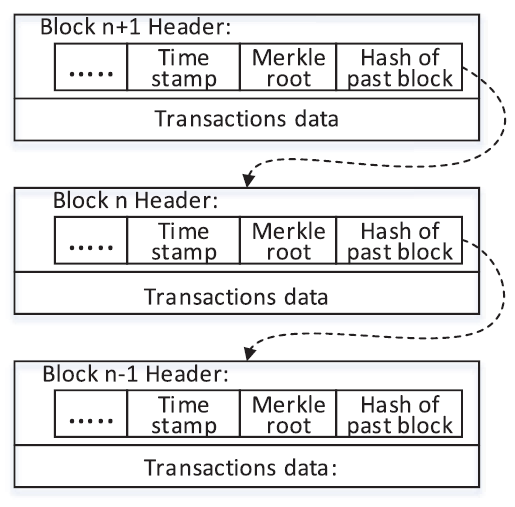
\includegraphics[height=0.20\textheight]{figures/Blockchain_Structure.png}
    \caption{\scriptsize Blockchain Structure~\cite{sanka2021systematic}}
    \label{fig:blockchain_structure}
  \end{subfigure}
  \hfill
  \begin{subfigure}[b]{0.45\linewidth}
    \centering
    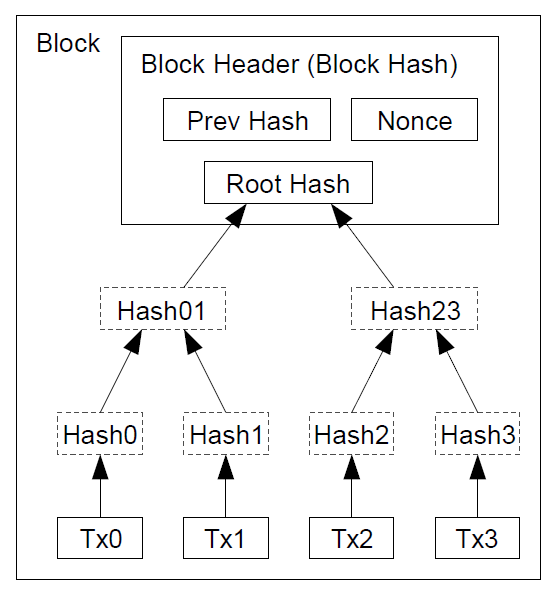
\includegraphics[height=0.20\textheight]{figures/Merkle_Tree.png}
    \caption{\scriptsize Merkle Tree~\cite{nakamoto2008bitcoin}}
    \label{fig:merkle_tree}
  \end{subfigure}
  \caption{Illustration of the blockchain structure and Merkle tree.}
  \label{fig:blockchain_overview}
\end{figure}
\vspace{12pt}

An overview of the blockchain structure (Fig.~\ref{fig:blockchain_structure}), as depicted in many visual representations, reveals that each block typically contains a block header and several transaction data~\cite{khan2021challenges}. For instance, a Bitcoin block can hold approximately 2000 transactions~\cite{nakamoto2008bitcoin}. The block header is crucial and comprises elements such as the hash of the previous block, a timestamp, the Merkle root of transactions, and a nonce, among other network-dependent components~\cite{khan2021challenges}. The Merkle root (illustrated in Fig.~\ref{fig:merkle_tree}) is a single hash value derived by continuously hashing all transactions within the block in pairs until only one root hash remains. This Merkle root protects the transaction data from tampering, as any alteration to the transaction data would change the Merkle root’s value~\cite{khan2021challenges}.

\vspace{12pt}
\subsubsubsection{Consensus Protocols}
\vspace{12pt}

The operational backbone of a blockchain network, particularly for creating new blocks and maintaining the network, lies in its consensus protocol [7], [8]. A consensus protocol defines the agreed-upon rules for how the network is maintained and, crucially, how the creator of a new block is selected [7].
Several consensus mechanisms exist, each with its own characteristics and trade-offs [7], [8], [11]:

Several consensus mechanisms exist, each with its own characteristics and trade-offs~\cite{khan2021challenges,zhou2020survey,aldoubaee2023review}:
\begin{itemize}
  \item \textbf{Proof of Work (PoW):} The most popular consensus protocol, first implemented in Bitcoin and also used by Ethereum. Special nodes called miners compete to solve a computational puzzle, and the first miner to succeed creates the new block. While PoW ensures strong security and decentralization, it suffers from low scalability and massive energy consumption~\cite{nakamoto2008bitcoin}.
  \item \textbf{Proof of Stake (PoS):} A less energy-intensive alternative where block creators (validators) are selected based on the amount of cryptocurrency they hold (stake)~\cite{buterin2014ethereum,zhou2020survey}.
  \item \textbf{Practical Byzantine Fault Tolerance (PBFT):} A voting-based protocol predominantly used in permissioned blockchains. It is valued for its scalability and Byzantine fault tolerance, but requires heavy messaging overhead~\cite{castro1999pbft}.
  \item \textbf{Raft:} A consensus protocol for permissioned blockchains, offering fault tolerance and high throughput, though it is not Byzantine fault-tolerant~\cite{ongaro2014raft}.
  \item \textbf{Other Mechanisms:} Variants such as Delegated Proof of Stake (DPoS), Proof of Elapsed Time (PoET), Tendermint, Ripple, Proof of Burn (PoB), Proof of Capacity (PoC), and Proof of Authority (PoA) are also widely studied~\cite{zhou2020survey}.
\end{itemize}

\vspace{12pt}

\subsubsubsection{Types of Blockchain}

\vspace{12pt}

Blockchains are typically classified into three main types based on their accessibility and participation models~\cite{sanka2021systematic}:

\begin{itemize}
    \item \textbf{Public Blockchain (Permissionless):} These networks are open to anyone. Any individual can join the network without prior permission, and participants have full rights to read and write blockchain data and participate in the network consensus. Examples include Bitcoin~\cite{nakamoto2008bitcoin} and Ethereum~\cite{buterin2014ethereum}. Public blockchains are highly decentralised and transparent, fostering trust among participants as everyone works towards improving the network. However, their open nature makes them more vulnerable to scalability issues as the number of users and transactions increases.

    \item \textbf{Private Blockchain (Permissioned):} In contrast, private blockchains require participants to have prior approval to join the network. This type of network is typically centralised and often owned by a single organisation, where all nodes are known and authorised. Examples include Multichain and BlockStack.

    \item \textbf{Consortium Blockchain (Permissioned):} Similar to private blockchains, consortium blockchains also require authorisation for participants to join the network, and their members are known. However, this type of network is formed by a group of organisations (a consortium) that seek to share data, often with little to no inherent trust among their members. A consortium blockchain is partially centralised. Hyperledger Fabric and Corda are notable examples.
\end{itemize}

\vspace{12pt}
\subsubsubsection{Conceptual Model for Blockchain Ecosystem}
\vspace{12pt}

To better describe the various components and architecture of a blockchain system, a five-layer conceptual model for the blockchain ecosystem has been proposed, drawing an analogy to networking models like OSI and TCP/IP. This model categorises the collection of components and services that together constitute blockchain technology:

\begin{figure}[htbp]
  \centering
  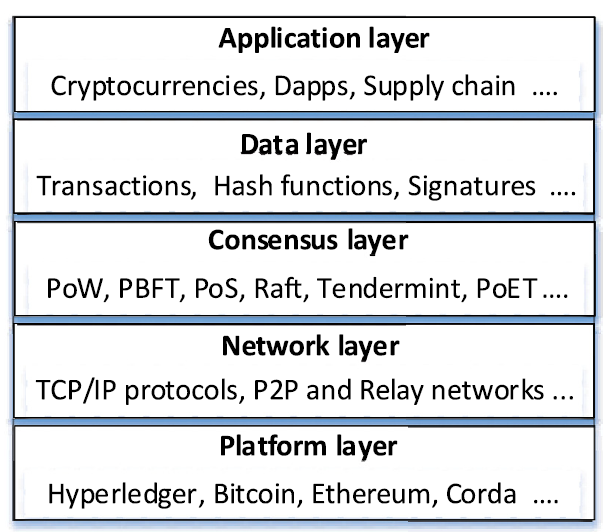
\includegraphics[width=0.4\linewidth]{figures/Poposed_Conceptual_Model_for_Blockchain_Ecosystem.png}
  \caption{\scriptsize Conceptual Model for Blockchain Ecosystem~\cite{sanka2021systematic}}
  \label{fig:Conceptual-Model-for-Blockchain-Ecosystem}
\end{figure}
\vspace{12pt}

\begin{itemize}
    \item \textbf{Application Layer:} This is the topmost layer, comprising the applications and use cases for which blockchain networks are created. These are the end products that deliver actual value to the end-user, such as cryptocurrencies, Decentralised Applications (DApps), and supply chain management systems.

    \item \textbf{Data Layer:} This layer consists of the fundamental components that form the blockchain data itself and the cryptographic protocols used for its creation and verification. It includes data structures, transactions, block headers, databases, hashing algorithms, digital signatures, and zero-knowledge proofs. This layer provides the basic ingredients for ensuring the integrity and authenticity of blockchain data.

    \item \textbf{Consensus Layer:} Responsible for providing the consensus protocols that manage and maintain the blockchain network. This layer dictates how new blocks are added and how the network achieves agreement. Key protocols here include Proof of Work (PoW) for public blockchains and Practical Byzantine Fault Tolerant (PBFT) for enterprise blockchains, alongside many others like Proof of Stake (PoS) and Tendermint.

    \item \textbf{Network Layer:} This layer encompasses the protocols and services for propagating blockchain data and messages among network participants, essentially providing the means of communication. Components include networking protocols (e.g., TCP/IP, gossip), networking software/hardware infrastructures (network stack, MAC), peer-to-peer networks, relay networks, and data propagation algorithms (e.g., data compression).

    \item \textbf{Platform Layer:} This foundational layer provides the blockchain software and hardware framework and infrastructure that integrates the functionalities of the layers above it. It serves as the technological backbone, with various blockchain vendors offering specific frameworks. Examples include Hyperledger Fabric, Bitcoin, Ethereum, and Multichain.
\end{itemize}

This layered model provides a structured approach to understanding where various scalability solutions can be applied within the complex blockchain ecosystem.

\vspace{12pt}
\subsubsubsection{The Blockchain Trilemma and Quadrilemma}
\vspace{12pt}

A foundational concept in blockchain design is the blockchain trilemma (Fig.~\ref{fig:trilemma}), introduced by Vitalik Buterin~\cite{buterin2014ethereum}. Similar to the CAP theorem in distributed systems~\cite{gilbert2002brewer}, the blockchain trilemma highlights the inherent trade-offs among three essential properties of a blockchain system: \textit{security}, \textit{scalability}, and \textit{decentralization}~\cite{zhou2020solutions}. It asserts that no blockchain can fully optimize all three simultaneously; instead, systems typically achieve two at the expense of the third.
\vspace{12pt}
For instance, Bitcoin—the pioneering blockchain—prioritizes security and decentralization to ensure tamper-resistance and censorship-resistance. However, this comes at the cost of scalability, resulting in relatively low transaction throughput~\cite{khan2021challenges}. Conversely, attempts to improve scalability often rely on a smaller number of more powerful nodes, which inherently reduces decentralization~\cite{chen2024survey}. Similarly, increasing throughput and confirmation speed to enhance scalability can inadvertently weaken security, introducing new vulnerabilities~\cite{chen2024survey}.

The trilemma is therefore not merely descriptive but a fundamental design constraint: no blockchain can maximize all three properties simultaneously. Instead, each system optimizes for two pillars while compromising the third, depending on the requirements of its intended application. Recognizing this trade-off is essential when evaluating scalability solutions, as it shapes what can realistically be considered “success” in decentralized systems.

\begin{figure}[htbp]
  \centering
  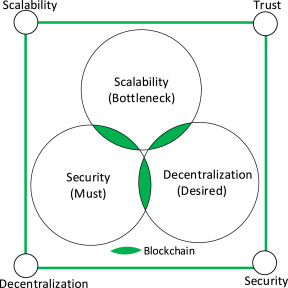
\includegraphics[width=0.55\linewidth]{figures/Blockchain_Scalability_Trilemma_Quadrilemma_Diagram.jpg}
  \caption{\scriptsize The Blockchain Trilemma and Quadrilemma~\cite{sanka2021systematic}}
  \label{fig:trilemma}
\end{figure}
\vspace{12pt}

Building upon this, researchers have expanded the concept into the blockchain \textit{quadrilemma} (also illustrated in Fig.~\ref{fig:trilemma}). This framework adds a fourth critical dimension—\textit{trust}—to the traditional trilemma of scalability, security, and decentralization~\cite{sanka2021systematic}. The quadrilemma reflects the inherent difficulty in simultaneously achieving all four properties, since improving one aspect often diminishes another. For example:

\begin{itemize}
    \item \textbf{Public blockchains} (e.g., Bitcoin, Ethereum) emphasize security and decentralization but sacrifice scalability.
    \item \textbf{Private and consortium blockchains} achieve higher scalability and security through trusted parties, but at the expense of decentralization.
    \item \textbf{DAG-based blockchains} can offer scalability and decentralization but may suffer from weaker security and reduced inherent trust~\cite{sanka2021systematic}.
\end{itemize}

Thus, the trilemma and quadrilemma together emphasize the inevitable trade-offs that shape blockchain architecture. They underscore that scalability challenges cannot be analyzed in isolation but must be assessed in relation to security, decentralization, and trust.

\vspace{12pt}
\subsubsection{Defining Blockchain Scalability}
\vspace{12pt}

Blockchain scalability refers to the ability of a blockchain network to efficiently process increasing volumes of transactions and user demand without undermining its foundational principles of security and decentralization~\cite{buterin2014ethereum,khan2021challenges}.

\vspace{12pt}
\subsubsubsection{Key Metrics for Evaluation}
\vspace{12pt}

Scalability is primarily assessed through technical metrics that directly influence system performance:

\begin{itemize}
    \item \textbf{Transactions per Second (TPS):} Measures throughput, i.e., how many transactions a blockchain can process per second. Higher TPS increases efficiency and reduces congestion~\cite{khan2021challenges,lin2024status}.
    \item \textbf{Latency (L):} The time required for a transaction to be confirmed and finalized. Low latency ensures faster processing and improves user experience~\cite{buterin2014ethereum,ledger2023tps}.
    \item \textbf{Block Size:} Determines how much data a block can hold. Larger blocks enable higher TPS but may increase propagation delay~\cite{buterin2014ethereum}.
    \item \textbf{Block Time:} The average time to generate a new block, directly impacting both throughput and latency~\cite{khan2021challenges}.
\end{itemize}

These metrics form the core benchmarks for comparing blockchain platforms and scaling mechanisms.

\vspace{12pt}
\subsubsubsection{Key Performance Indicators (KPIs)}
\vspace{12pt}

Beyond raw technical metrics, broader system-level KPIs provide insights into the operational scalability and reliability of blockchain implementations:

\begin{itemize}
    \item \textbf{Network Uptime and Availability:} Ensures continuous operation without downtime~\cite{slogix2025scalability}.
    \item \textbf{Data Integrity and Immutability Verification:} Validates that records remain tamper-proof and trustworthy~\cite{slogix2025scalability}.
    \item \textbf{Smart Contract Vulnerability Rate:} Measures the security and robustness of programmable components~\cite{slogix2025scalability}.
\end{itemize}

These KPIs complement technical metrics by capturing practical reliability and security aspects, which are crucial for real-world adoption.


\vspace{12pt}
\subsection{Problem Statement}
\vspace{12pt}

The overarching problem addressed by this research is the scalability issue in blockchain technology, which significantly hampers its broader adoption and limits its potential across various applications. Despite blockchain's compelling advantages—such as enhanced security, decentralisation, and immutability—its current performance characteristics fall short of the demands of high-volume, real-world systems, leading to a critical bottleneck.

Specifically, the scalability problem manifests through several key performance deficiencies:

\subsubsection*{Low Transaction Throughput and Latency (Write-Performance)}
Major public blockchains, such as Bitcoin (3--4 TPS) and Ethereum ($\sim$15 TPS), process transactions at speeds orders of magnitude lower than centralised payment networks like Visa ($\sim$1667 TPS) or PayPal ($\sim$193 TPS)~\cite{x}. This limited processing capacity leads to network congestion when user demand increases, making the systems impractical for high-frequency transactions.

Beyond throughput, the time taken for a transaction to be confirmed and added to the blockchain (latency) is often substantial. Bitcoin transactions, for instance, can require six confirmations (approximately one hour) for security reasons. The average waiting time for a transaction to be validated can increase to 29 minutes~\cite{ref5}. These delays make blockchain unsuitable for applications requiring instant finality, such as real-time payments or dynamic gaming environments.

\subsubsection*{Low Read Throughput and Latency (Read-Performance)}
Beyond transaction writes, blockchain scalability is constrained by poor read-performance. Lightweight nodes---such as Simplified Payment Verification (SPV) clients, IoT devices, or intermittently connected peers---do not maintain the full ledger and must query full blockchain nodes for data.

Read throughput refers to the number of queries a full node can process per second, while read latency measures the time taken for a data request to be fulfilled. In current systems, both remain suboptimal due to the sheer size of the blockchain and the absence of efficient indexing or standardized query languages. This leads to slow data access, which restricts blockchain’s applicability in data-intensive or real-time applications (e.g., supply-chain tracking, healthcare monitoring, or IoT event validation) and imposes heavy loads on full nodes~\cite{sanka2021systematic}.

\subsubsection*{Storage Requirements (Storage-Performance)}
As append-only ledgers, blockchains grow continuously. By March 2023, the Bitcoin blockchain exceeded 465~GB, while Ethereum grew beyond 1~TB~\cite{sanka2021systematic,nakamoto2008bitcoin}. More recently, the Bitcoin ledger has expanded further to approximately 679.5~GB as of August 2025 (see Fig.~\ref{fig:blockchain_growth})~\cite{ref6}.

\begin{figure}[h!]
  \centering
  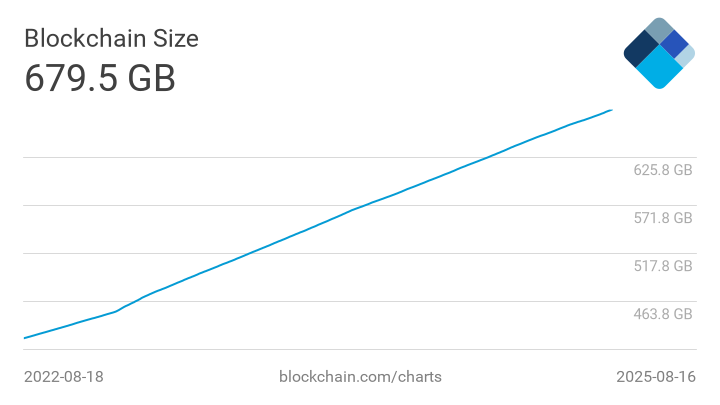
\includegraphics[width=0.7\textwidth]{figures/blocks-size.png}
  \caption{Growth of the Bitcoin blockchain size (2018--2025).}
  \label{fig:blockchain_growth}
\end{figure}

This enormous data footprint makes full-node participation impractical for lightweight devices such as IoT nodes, smartphones, or embedded systems, thereby restricting blockchain’s integration into resource-constrained environments.

\subsubsection*{Economic Costs (High Transaction Fees)}
Periods of network congestion directly correlate with increased transaction fees, as users compete for limited block space. This dynamic makes small or frequent operations economically unviable for many users and discourages the wider use of blockchain technology in everyday applications, particularly in decentralised finance (DeFi) and gaming where cost-effectiveness is critical.

\subsubsection*{Research Gap}
Existing research efforts to address scalability often focus on specific solutions in isolation, such as sharding, and frequently overlook other critical aspects like read-performance or comprehensive storage solutions. There is a recognised gap in providing a systematic, holistic review that assesses the current state-of-the-art across all dimensions of scalability, their practical implementations, and their measured performance in real-world or simulated environments.

\bigskip

Without effective solutions to these multifaceted scalability challenges, blockchain technology will remain limited in its capacity to handle large transaction volumes efficiently, restricting its widespread adoption and preventing it from fully realising its transformative potential in high-demand applications. Therefore, a systematic and in-depth investigation into current and emerging scalability solutions, their performance, trade-offs, and future directions, is urgently needed.

\subsection{Research Questions}
\vspace{12pt}
\begin{enumerate}
    \item \textbf{How can we accurately predict the necessary resources for container startup without relying on runtime data?}
    
    \begin{itemize}
        \item What factors influence the resource requirements at container startup?
        \item How can we model these factors to predict resource needs?
        \item Can we leverage historical data from similar containers to improve prediction accuracy?
    \end{itemize}
    
    \item \textbf{What is the optimal duration for applying a resource boost to a container at startup?}
    
    \begin{itemize}
        \item How can we determine the initial boost duration without runtime data?
        \item What methods can be used to dynamically adjust the boost duration based on observed container behavior during startup?
        \item How does the boost duration impact overall system performance and resource efficiency?
    \end{itemize}
    
\end{enumerate}

\subsection{Research Objectives}
\vspace{12pt}
\begin{enumerate}
    \item \textbf{Develop a predictive model for initial resource allocation:}

\begin{itemize}
    \item Create a model that can predict the necessary resources for container startup based on factors like container characteristics, and historical data from similar images without relying on runtime data.
    \item Validate the model’s predictions against actual resource usage at startup to provide improved predictions overtime.
\end{itemize}

    \item \textbf{Establish a methodology for determining the optimal boost duration:}

\begin{itemize}
    \item Investigate different strategies for setting the initial boost duration, including static time periods and dynamic adjustments based on startup behavior.
    \item Assess the impact of various boost durations on container performance and overall resource utilization.
    
\end{itemize}

\item Propose an integrated approach that combines initial allocation predictions with ongoing runtime optimizations\cite{tran2022survey} to improve resource management throughout the container life-cycle. (Optional)
\end{enumerate}

\vspace{12pt}
These objectives aim to provide a comprehensive framework for optimizing resource allocation at container startup, improving both the efficiency and performance of containerized applications.



\vspace{12pt}

\subsection{Research Outcomes}
\vspace{12pt}
The primary outcome of this research is to achieve an optimized startup process for containerized applications using a novel self-adaptive CPU allocation system through the effective implementation of Kube Startup CPU Boost. This outcome has several facets:

\begin{enumerate}
    \item \textbf{Faster Application Startup}:
By temporarily increasing CPU resources during the startup phase, applications can perform necessary operations such as class loading, just-in-time compilation, and initial code optimization more quickly. This results in significantly reduced startup times, which is particularly beneficial for resource-intensive applications like those built on Java Virtual Machines (JVMs).

    \item \textbf{Improved Resource Utilization}:
Efficient resource allocation ensures that containers are provisioned with just the right amount of CPU during their critical startup phase, meeting their high initial demand without overprovisioning. Once this phase is over, the resources are dynamically scaled down to match normal usage, avoiding underprovisioning. This dynamic adjustment leads to improved overall resource utilization across the Kubernetes cluster, ensuring that resources are used optimally and efficiently throughout the lifecycle of the pods.

    \item \textbf{Enhanced User Experience}:
Faster startup times and stable application performance translate to a better user experience. Applications become more responsive, leading to higher user satisfaction and retention.

    \item \textbf{Reduced Operational Overhead}:
Automating the initial resource allocation process through predictive models and dynamic adjustments decreases the manual effort required by platform engineers. This allows engineering teams to focus on more strategic tasks rather than constant resource tuning.

    \item \textbf{Cost Savings}:
Optimizing resource allocation reduces cloud infrastructure costs by minimizing wasted resources. The use of startup cpu boost and runtime vertical scaling by leveraging predictive algorithms to allocate resources precisely when needed, businesses can achieve substantial cost savings without compromising application performance.

\end{enumerate}
In conclusion, the optimized startup of containers using Kube Startup CPU Boost and predictive algorithms addresses critical challenges in resource management, leading to faster, more efficient, and cost-effective application deployment and operation.
Further this research can also be extended to resource constrained and time sensitive environments such as server-less deployments and embedded systems.
\newpage

\section{Literature Review}

The current body of research on blockchain scalability is extensive, yet often fragmented. Existing surveys frequently focus on specific aspects, such as sharding, leaving other critical dimensions like read-performance, storage solutions, and comprehensive performance analysis underexplored. This literature review aims to provide a broader and more systematic overview, based on the proposed five-layer blockchain ecosystem model~\cite{ref1} (Data, Consensus, Network, Platform, and Application layers) and exploring both write-performance, read-performance, and storage scalability solutions, along with their empirical performance metrics and identified limitations.

\subsection{Write-Performance Scalability Solutions}
Write-performance, primarily measured by transaction throughput (TPS) and transaction latency, is a critical aspect of blockchain scalability. Solutions in this area aim to increase the rate at which transactions are processed and confirmed.

\subsubsection{Data Layer Solutions (On-Chain)}
On-chain solutions involve modifications to the main blockchain structure itself.

\paragraph{Reducing Block Data}
This approach focuses on optimising the content within blocks to accommodate more transactions without excessively increasing the physical block size.

\textbf{SegWit (Segregated Witness):} Separates signature data from transaction data and appends it as metadata, effectively freeing up space within the block. This allows for approximately four times more transactions per block and increases Bitcoin's effective block size from 1 MB to 4 MB. It also addresses transaction malleability and facilitates off-chain solutions like the Lightning Network. However, its throughput improvement is limited to 17–23 TPS. It also caused a hard fork in Bitcoin and requires further scaling efforts.

\textbf{Merkelized Abstract Syntax Tree (MAST):} A Bitcoin Improvement Proposal (BIP-114) that represents Bitcoin scripts as a Merkle tree of their Abstract Syntax Tree (AST) branches. This allows unused sub-scripts to be removed from a block, achieving substantial block size reduction on a logarithmic scale.

\textbf{Lumino Transaction Compression Protocol (LTCP):} Used in the RSK network, LTCP employs delta compression to remove selected fields (e.g., some signatures) from a block, resulting in up to 90\% block data reduction. It aims to scale the RSK network to 2000 TPS and could potentially scale Bitcoin to 100 TPS.

\paragraph{Directly Increasing Block Size}
\textbf{Bitcoin-Cash (BCH) and Bitcoin-Unlimited (BU):} Following the SegWit soft fork, Bitcoin-Cash emerged as a hard fork, initially increasing the Bitcoin block size limit to 8 MB and later to 32 MB. While this increases transaction capacity, direct increases in block size can introduce security vulnerabilities due to increased propagation delays, potentially leading to more forks and denial-of-service (DoS) attacks. It can also raise centralisation concerns.

\textbf{Litecoin:} With a 2.5-minute block interval, faster than Bitcoin's 10 minutes, Litecoin achieves 56 TPS. However, this faster block generation can lead to more orphaned blocks due to time lags in acceptance.

\paragraph{Sharding}
A technique adapted from distributed database systems, sharding divides the blockchain network into smaller, independent groups called shards. Each shard processes transactions and stores data in parallel, thereby scaling the blockchain horizontally.

Examples include:
\begin{itemize}
  \item \textbf{Elastico:} Throughput of 40 TPS with 1600 nodes; limited fault tolerance (25\%).
  \item \textbf{Omniledger:} Uses ByzCoinX consensus; 3500 TPS with 600 nodes/shard; vulnerable to DoS.
  \item \textbf{RapidChain:} No trusted setup; 7300 TPS, 8.7s confirmation with 4000 nodes; prone to partitioning.
  \item \textbf{Monoxide:} 11,694 TPS with 48,000 nodes; concerns over miner centralisation.
  \item \textbf{Ethereum 2.0 Sharding:} Aims for 100,000 TPS with 64 shards and hybrid BFT-PoS.
  \item \textbf{Ostraka:} Node-level sharding; significant throughput improvement, but bandwidth not sharded.
\end{itemize}

\paragraph{Directed Acyclic Graph (DAG) Solutions}
\begin{itemize}
  \item \textbf{Conflux:} 6400 TPS, 4.5–7.4 min confirmation.
  \item \textbf{Tangle (IOTA):} $>$1000 TPS; coordinator node raises centralisation/security concerns.
  \item \textbf{ByteBall:} Witness-based validation; 20 TPS.
  \item \textbf{Spectre:} Concurrent mining, tolerant to 50\% adversaries.
  \item \textbf{CoDAG:} Compacted DAG achieving 394 TPS.
\end{itemize}

\paragraph{Parallel Executions (Smart Contracts)}
Random assignment, contract partitioning, and multi-threading enable parallel smart contract execution.

\subsubsection{Data Layer Solutions (Off-Chain)}
Transactions or tasks are conducted outside the main blockchain, with only summaries recorded on-chain.

\paragraph{Payment and State Channels}
\textbf{Lightning Network (Bitcoin):} Instant micropayments with claims of 40M TPS, limited to small values and online parties.  
\textbf{Raiden Network (Ethereum):} Similar to Lightning, supports ERC20 tokens.

\paragraph{Sidechains}
\textbf{Plasma (Ethereum):} Smart contract sidechains, potentially 100x faster than Ethereum.  
\textbf{ZK-Rollup:} 2000–3000 TPS; data availability and centralisation risks.  
\textbf{Liquid Network (Bitcoin):} 2-min block finality via Strong Federation.  
\textbf{RootStock (RSK):} Smart contracts on Bitcoin; 300–1000 TPS.

\paragraph{Cross-Chains}
\textbf{Cosmos:} IBC protocol, Tendermint consensus.  
\textbf{Polkadot:} Relay-chain with parachains for interoperability and scalability.

\paragraph{Off-Chain Computations}
\textbf{TrueBit (Ethereum):} Offloads heavy computations with verifiable proofs.  
\textbf{Arbitrum (Ethereum):} Executes smart contracts off-chain; main chain only verifies signatures.

\subsubsection{Consensus Layer Scalability Solutions}
\paragraph{PoW Improvements}
\textbf{Bitcoin-NG:} 10x TPS via microblocks.  
\textbf{GHOST:} Improves Bitcoin throughput to 200 TPS.

\paragraph{PoS Improvements}
\textbf{DPoS:} $>$2000 TPS but raises centralisation concerns.  
\textbf{Ouroboros:} Cardano’s secure PoS.

\paragraph{BFT Improvements}
\textbf{PBFT:} $>$1000 TPS in private chains, but $O(N^2)$ overhead.  
\textbf{Tendermint:} 10,000 TPS, tolerates 1/3 adversaries.  
\textbf{SBFT/T-PBFT:} Reduce communication overhead.

\paragraph{Hybrid Protocols}
\textbf{Ethereum Casper:} Combines PoS + BFT.  
\textbf{ByzCoin:} PoW + PBFT, 1500 TPS.  
\textbf{Algorand BA:} Confirmation $<$1 min, 125x Bitcoin throughput.

\subsubsection{Network Layer Scalability Solutions}
\paragraph{Relay Networks}
\textbf{Fiber, GeeqChain:} Reduce propagation delays but raise centralisation concerns.

\paragraph{RINA}
Cardano’s alternative to TCP/IP for faster propagation.

\paragraph{RDMA Networking}
High-performance communication bypassing CPU/OS.

\paragraph{Data Compression}
\textbf{Compact Block Relay (BIP152):} Saves bandwidth 10x.  
\textbf{Txilm:} 80x reduction using short hashes.

\subsubsection{Platform Layer Scalability Solutions}
\paragraph{Hyperledger Fabric}
Execute-Order-Validate architecture; FastFabric scales to 20,000 TPS.

\paragraph{Ethereum 2.0}
Casper-sharding + eWASM; targets 100,000 TPS.

\subsection{Storage Scalability Solutions}
\paragraph{Data Pruning and Compression}
Mini-Blockchain scheme deletes old tx; IoT-focused compression.

\paragraph{Off-Chain Storage}
\textbf{DHTs, IPFS (Filecoin, Disema):} Offload raw data.  
\textbf{CUB, Jidar:} Peer-based or trustless reduction.

\paragraph{Enhanced Databases}
\textbf{BigchainDB:} Millions of writes/sec, petabyte scale, NoSQL querying.

\subsection{Read-Performance Scalability Solutions}
\paragraph{Hardware Caching}
\textbf{FPGA caching:} Handles requests directly, reduces server load.

\paragraph{Improved Query}
\textbf{Ethereum Query Language (EQL):} SQL-like queries for Ethereum.

\subsection{Summary of Scalability Solutions \& Trade-offs}
On-chain solutions offer direct improvements but raise security and centralisation issues. Off-chain methods provide higher throughput and privacy but may require locked funds or introduce new attack vectors. Consensus, network, and platform-level solutions enhance performance but carry trade-offs in complexity, security, or interoperability. Storage and read-performance methods mitigate data and query inefficiencies.  
Overall, the \textbf{blockchain quadrilemma} persists: scalability, decentralisation, security, and trust cannot be simultaneously maximised. Each solution balances these dimensions differently, highlighting the need for context-specific trade-offs.

\newpage

\section{Methodology}

This research proposal adopts a systematic review approach to comprehensively investigate the current state-of-the-art in blockchain scalability. This methodology is chosen due to its rigorous and transparent nature, enabling a thorough and unbiased synthesis of existing research, identifying trends, solutions, performance metrics, and prevailing challenges. This systematic process ensures that all relevant aspects of blockchain scalability, including write-performance, read-performance, storage solutions, and performance analysis, are covered, addressing the limitations of prior reviews which often focus on narrow aspects.

\subsection{Research Design}
The research design is structured around a multi-stage systematic review process, as illustrated in the provided source (similar to Fig.~4 in Sanka \& Cheung). This process typically involves:
\begin{enumerate}
    \item Defining research questions,
    \item Identifying relevant studies,
    \item Selecting papers based on defined criteria,
    \item Extracting and synthesising data, and
    \item Reporting the findings.
\end{enumerate}

The primary objective is to build a thorough knowledge base in blockchain technology, specifically concerning solutions to scalability issues. By exploring the implementation and techniques of various state-of-the-art scalability solutions, this study aims to:
\begin{itemize}
    \item Provide a deeper understanding of these solutions,
    \item Construct a performance metric of listed scalability solutions,
    \item Evaluate the limitations encountered with the integration of these solutions.
\end{itemize}

\subsection{Data Collection Strategy}
The data collection strategy is designed to ensure comprehensive coverage of relevant literature from both academic and grey areas, following a robust, multi-phase approach.

\subsubsection{Database Selection}
To maximise the breadth of coverage, the search will be conducted across a selection of major, reputable science-related databases. These include:
\begin{itemize}
    \item IEEE Xplore
    \item ACM Digital Library
    \item ScienceDirect
    \item Springer Link
    \item Wiley Online Library
    \item Web of Science
    \item Google Scholar (particularly useful for capturing grey literature such as white papers and reports)
    \item Scopus
\end{itemize}

\subsubsection{Timeframe and Publication Types}
\begin{itemize}
    \item \textbf{Timeframe:} The search will cover publications released within the range of 2012--202X. This period captures the emergence of significant blockchain research and development beyond Bitcoin's initial phase.
    \item \textbf{Publication Types:} Conferences, Journals, White papers, Archives, Reports, Symposiums, Workshops, and Patents.
    \item \textbf{Language:} Only papers written in English will be included.
\end{itemize}

\subsubsection{Phase 2: Secondary Phase (Manual/Supplementary Search)}
Recognising that automated searches may miss some relevant papers, a manual, supplementary search will be conducted. This involves checking the references and citations of all papers selected in the primary phase. Additional relevant papers will then be added to the primary set.

\textbf{Inclusion Criteria:} Papers directly addressing blockchain scalability issues, proposing solutions, conducting performance analyses, or reviewing scalability aspects. Focus on public blockchain platforms. \\
\textbf{Exclusion Criteria:} Papers not directly related to blockchain scalability, short abstracts or posters without substantial content, duplicate entries, or non-English publications.

\subsection{Data Analysis and Synthesis}
The selected papers will undergo a systematic data extraction and synthesis process to address the research questions and achieve the objectives.

\subsubsection{Classification Framework}
All selected papers will be classified using a multi-tiered framework derived from the proposed five-layer conceptual model for the blockchain ecosystem:
\begin{itemize}
    \item \textbf{Main Categories:}
    \begin{itemize}
        \item Scalability Solution Proposals
        \item Performance-Analysis Studies
        \item Review/Survey Papers
    \end{itemize}
    \item \textbf{Sub-Classification of Scalability Solutions:}
    \begin{itemize}
        \item Write-Performance Solutions: On-Chain (reducing block data, increasing block size, sharding, DAG, parallel executions) and Off-Chain (payment channels, sidechains, cross-chains, off-chain computations).
        \item Consensus Layer Solutions: probabilistic, non-probabilistic, hybrid.
        \item Network Layer Solutions: network structure improvements, data compression, other optimisations.
        \item Platform Layer Solutions: platform-specific (e.g., Hyperledger Fabric, Ethereum 2.0).
        \item Read-Performance Solutions.
        \item Storage Solutions.
    \end{itemize}
    \item \textbf{Sub-Classification of Performance Analysis Studies:}
    \begin{itemize}
        \item Modelling Analysis Studies,
        \item Benchmarking Studies,
        \item Performance Evaluation Studies.
    \end{itemize}
\end{itemize}

\subsubsection{Performance Metric Construction and Comparative Analysis}
For each identified scalability solution, relevant performance data will be extracted and compiled to construct a comprehensive performance metric. Key performance indicators (KPIs)\cite{your-kpi-source} to be analysed include:
\begin{itemize}
    \item Transaction Throughput (TPS),
    \item Transaction Latency (confirmation time),
    \item Data Read Throughput/Latency,
    \item Data Storage Volume,
    \item Security and Decentralisation implications,
    \item Energy Consumption.
\end{itemize}

A comparative analysis will then be performed, highlighting strengths, weaknesses, and trade-offs (e.g., improved throughput at the cost of decentralisation).

\subsubsection{Qualitative Analysis and Identification of Research Gaps}
Beyond quantitative metrics, a qualitative assessment will be conducted focusing on:
\begin{itemize}
    \item Underlying mechanisms and technological approaches,
    \item Applicability to public, private, and consortium blockchains,
    \item Practical challenges during implementation,
    \item Extent to which solutions address the blockchain quadrilemma.
\end{itemize}

Finally, critical research gaps and future opportunities will be identified, including the need for:
\begin{itemize}
    \item More robust benchmarking tools,
    \item Innovative hybrid scalability solutions,
    \item Greater exploration of under-researched areas (e.g., read-performance, holistic storage solutions).
\end{itemize}

\newpage

\section{Evaluation}
\input{chapters/4-evaluation}
\newpage

\section{Research Timeline}
This section outlines the timeline for the project, including the various phases, key milestones, and the overall schedule depicted in the Gantt chart. The timeline is designed to ensure the project progresses smoothly and all deliverables are met within the specified timeframe.

\vspace{12pt}
\subsection{Project Phases}
\vspace{12pt}

The key project phases are structured to guide the project from initiation to completion. Each phase has specific objectives and tasks that contribute to the successful delivery of the project. The phases are:
\begin{enumerate}
    \item Project Initiation: Conducting the Literature Review, Defining the project scope, objectives, and deliverables.
    \item Tool Selection and Setup: Identifying and configuring the necessary tools and technologies.
    \item Implementation: Developing and integrating the project components.
    \item Evaluation: Testing and validating the project's outcomes.
    \item Documentation and Presentation: Preparing the final documentation and presenting the project results.
\end{enumerate}

\vspace{12pt}
\subsection{Milestones}
\vspace{12pt}

To monitor progress and ensure timely completion, the project includes several key milestones. These milestones mark significant points in the project and serve as checkpoints to review progress. The milestones are:
\begin{enumerate}
    \item Literature Review Completion: Completing the review of relevant literature and research.
    \item Project Proposal Submission: Submitting the detailed project proposal.
    \item First Prototype: Developing and testing the initial prototype.
    \item Final Solution: Completing the final version of the project.
    \item Research Paper Submission: Submitting the research paper detailing the project outcomes.
    \item Final Report Submission: Submitting the comprehensive final report of the project.
\end{enumerate}

\vspace{12pt}
\subsection{Gantt Chart}
\vspace{12pt}

The following Gantt chart conveys the estimated timeline, project deliverables, and the planned stages of the project. It provides a visual representation of the project schedule and helps in tracking the progress of each phase and milestone.

\begin{figure}[htbp]
  \centering
  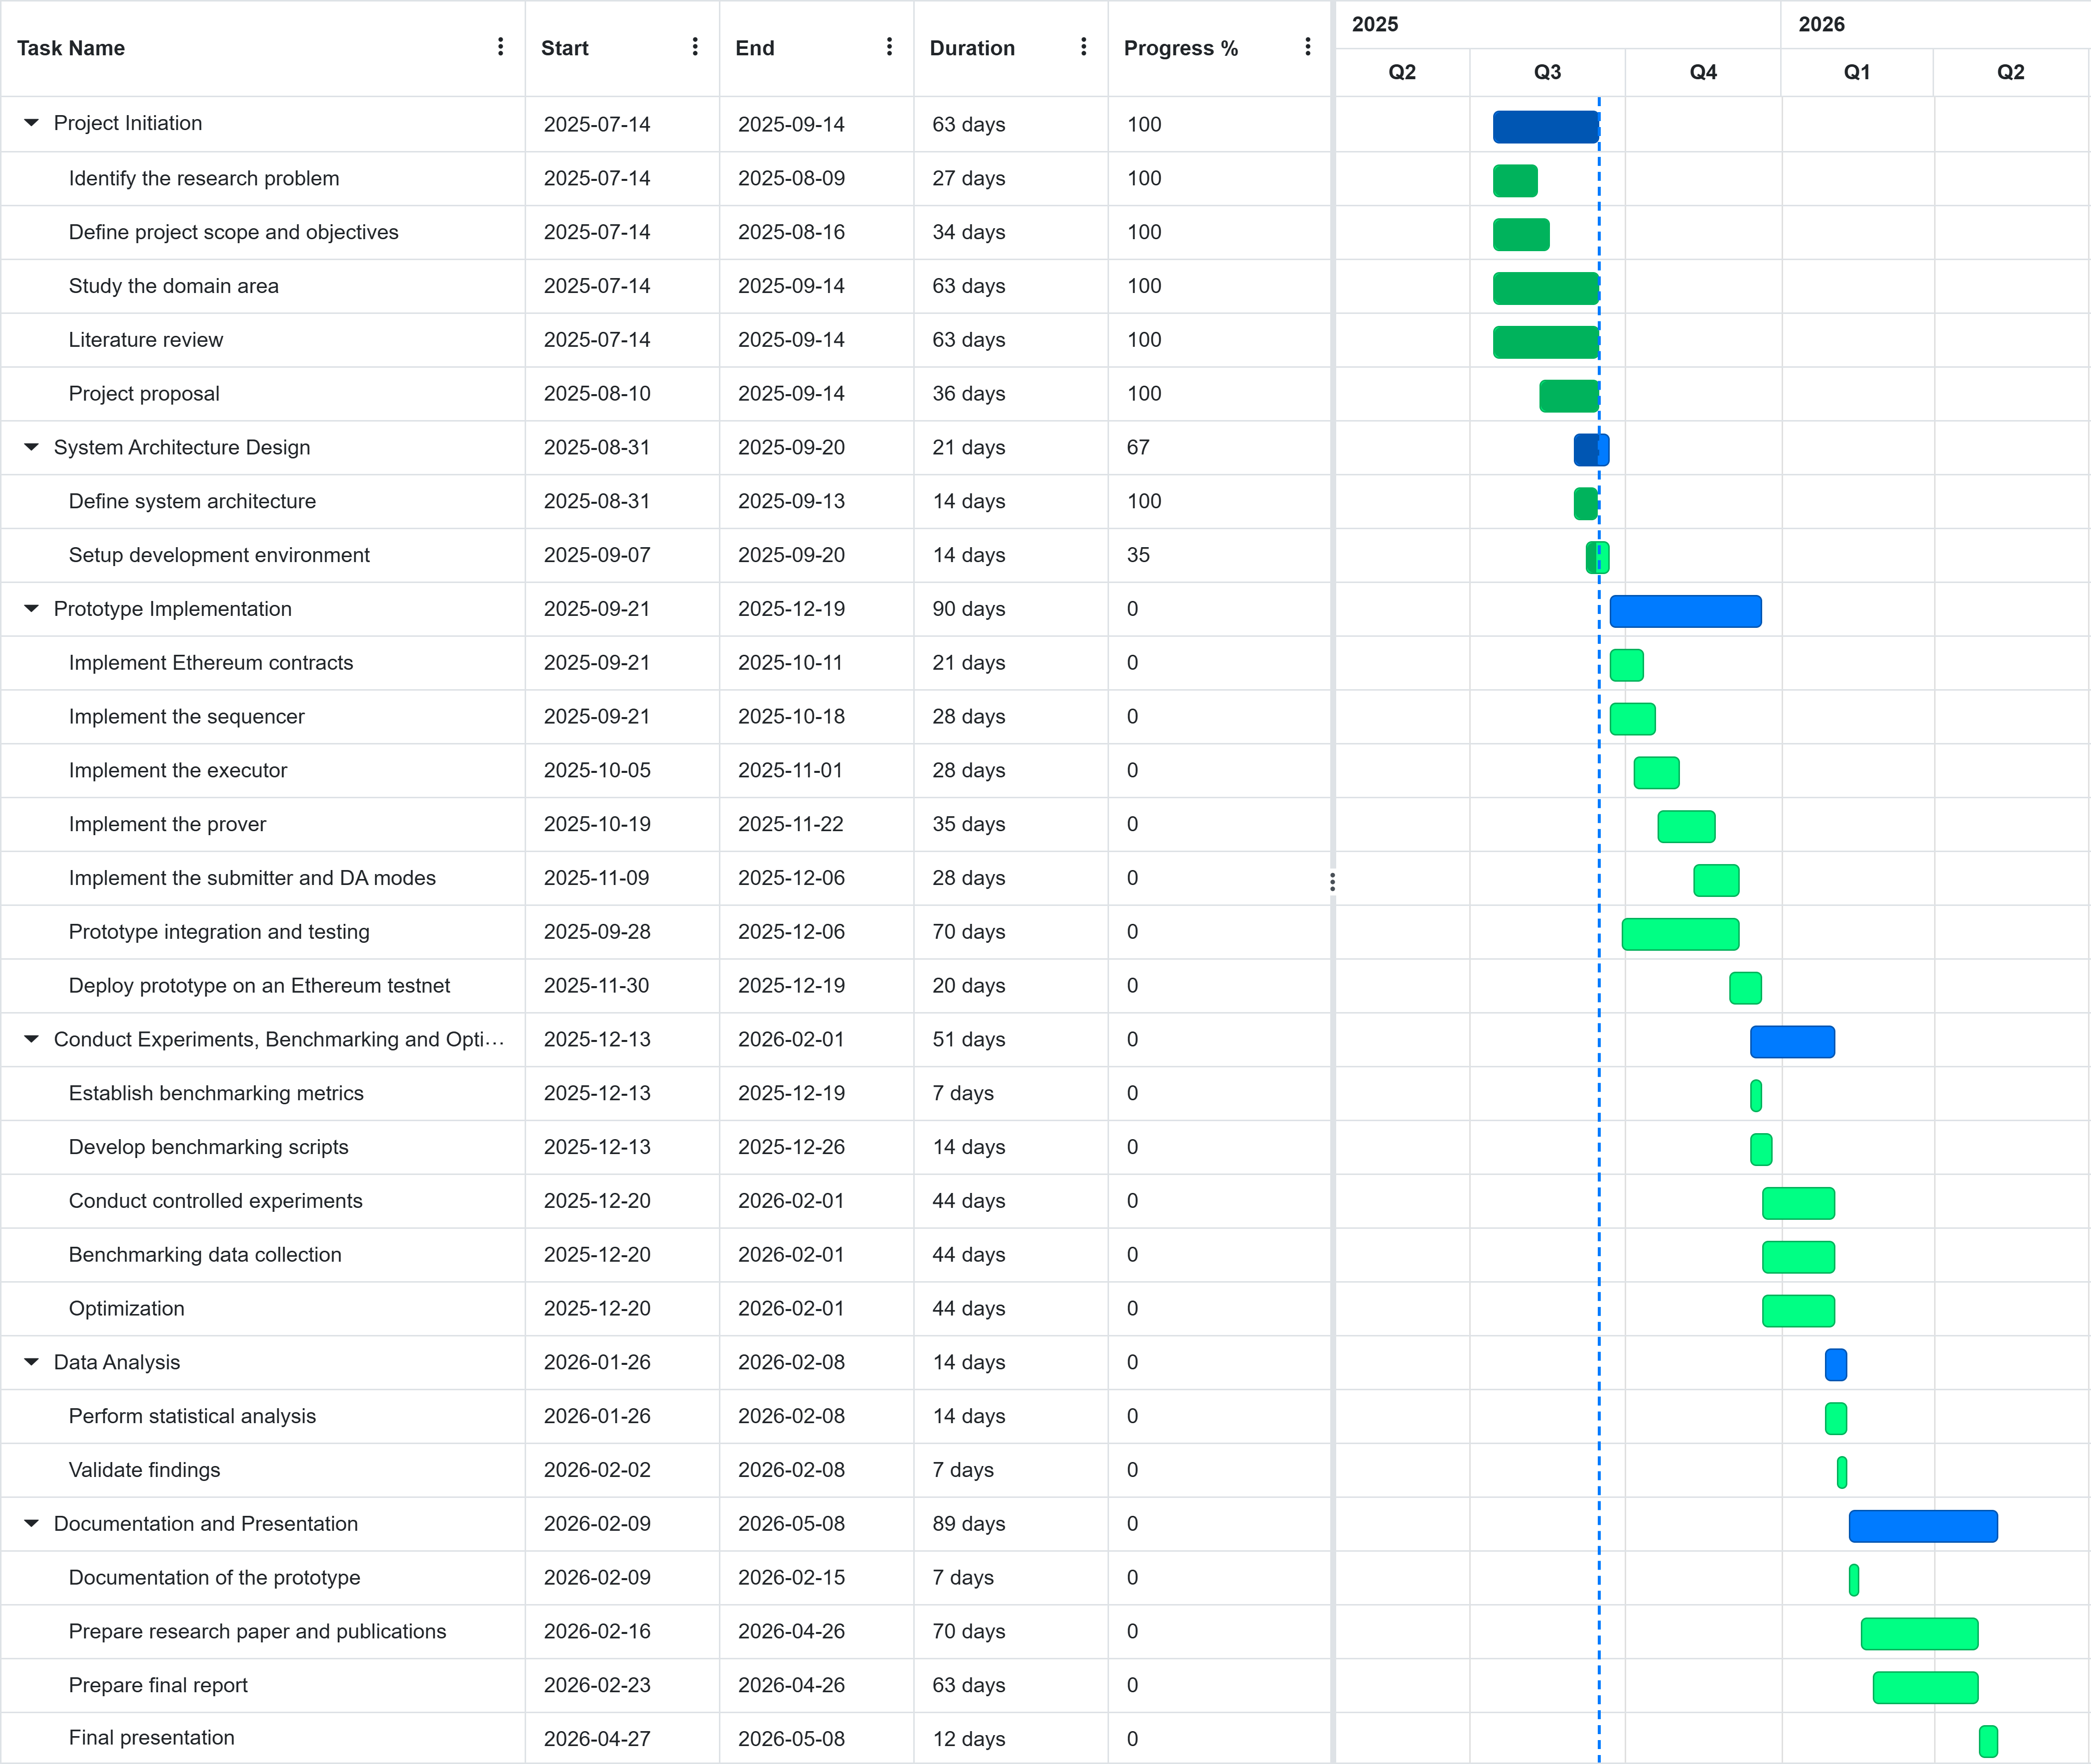
\includegraphics[height=0.8\linewidth, angle=90]{figures/proposed-timeline.png}
  \caption{Gantt Chart for the project timeline}
  \label{fig:operation-flow}
\end{figure}


\clearpage
\newpage

\section{Feasibility and Conclusion}
\subsection{Feasibility}
\vspace{12pt}

The proposed research on blockchain scalability is highly feasible, drawing upon a robust foundation of existing technologies, ongoing industry developments, and a strong market demand for enhanced blockchain performance.

\subsubsection{Technical Feasibility}
The extensive literature reviewed demonstrates that various technical approaches to blockchain scalability---including on-chain modifications (e.g., sharding, DAGs, block compression), off-chain solutions (e.g., payment channels, sidechains, cross-chains), advanced consensus mechanisms, and network/platform-layer optimisations---have been proposed, prototyped, and in some cases partially implemented. Frameworks such as Ethereum~2.0 and architectural advancements in Hyperledger Fabric exemplify the active pursuit of scalable blockchain solutions. These diverse methods confirm that improving blockchain performance is technically achievable, albeit complex, involving trade-offs. The feasibility of this research relies on synthesising these existing technical efforts rather than proposing entirely new, unproven technologies.

\subsubsection{Resource Availability}
Conducting a systematic review requires access to academic databases and literature management tools. The specified databases (IEEE Xplore, ACM Digital Library, ScienceDirect, Springer Link, Web of Science, Google Scholar, Scopus) are widely accessible within academic institutions. Tools like EndNote or Zotero are standard for managing references and screening papers, ensuring efficient execution of the methodology. Thus, the necessary informational and software resources are readily available.

\subsubsection{Data Availability}
The empirical performance metrics and analyses, as presented in the reviewed research, provide a rich source of data for comparative evaluation. Studies on throughput, latency, and storage, as well as qualitative assessments of security and decentralisation, are well documented. This ensures feasibility of the proposed analysis without requiring new data generation from scratch. These align closely with technical KPIs such as \textit{Transactions per Second (TPS)}, \textit{Transaction Latency}, \textit{Block Size/Time}, and \textit{Network Uptime}:contentReference[oaicite:2]{index=2}.

\subsubsection{Expertise}
The research builds upon established concepts in distributed ledger technologies, cryptography, computer networks, and performance analysis. Researchers with backgrounds in these fields---such as the authors of the provided sources (e.g., Sanka and Cheung, with expertise in blockchain technology, digital systems design, network computing, and information security)---possess the requisite knowledge to undertake such a comprehensive study.

\subsubsection{Societal and Economic Feasibility}
There is a significant and growing demand for scalable blockchain solutions across industries. The forecasted business value of blockchain (over \$3.1 trillion by 2030) and the high percentage of companies planning to integrate it underscore the economic incentive. Addressing scalability is crucial for blockchain to transition from experimental stages to mainstream production, enabling adoption in decentralised finance (DeFi), supply chain, healthcare, and IoT. This validates both the societal and economic relevance of the research.

\subsubsection{Current Adoption Trends}
The increasing adoption of blockchain by major companies (e.g., Microsoft, IBM, Oracle, Ford, BMW, Renault, Maersk) and countries (e.g., El-Salvador, Georgia, UAE, Singapore) for diverse applications demonstrates real-world demand. This ongoing integration across sectors indicates a sufficiently mature ecosystem to support further scalability research, making the study timely and impactful.

\subsection{Conclusion}
In conclusion, the proposed research is highly feasible, supported by existing technological advancements, readily available academic resources, a wealth of empirical data, and a clear market demand. By systematically synthesising state-of-the-art solutions and evaluating them against well-defined KPIs---spanning \textit{technical performance}, \textit{operational efficiency}, \textit{economic viability}, and \textit{security}:contentReference[oaicite:3]{index=3}:contentReference[oaicite:4]{index=4}---this study aims to provide a comprehensive understanding of blockchain scalability. The findings will contribute both theoretically and practically, guiding the design and adoption of scalable blockchain systems.



\vspace{12pt}
\subsection{Conclusion}
\vspace{12pt}

This project proposal outlines an innovative approach to optimize container startup times in Kubernetes environments through self-adaptive CPU allocation. By leveraging predictive algorithms and integrating with the Kube Startup CPU Boost feature, the project aims to significantly reduce application startup times and enhance resource allocation efficiency. The proposed solution addresses the critical challenge of efficient resource allocation during the resource-intensive startup phase of applications, combining real-time monitoring, predictive analysis, and startup boost to ensure optimal CPU allocation without over/under provisioning.

\vspace{12pt}

The potential impact of this project is substantial, with expected improvements in application performance, reduced operational/management costs, and enhanced overall efficiency of Kubernetes clusters. The comprehensive evaluation plan, including a range of benchmarks and performance metrics, will provide a thorough assessment of the solution's effectiveness. Given its technical viability and potential economic benefits, this project represents a significant step forward in container orchestration and resource management, with the potential to contribute valuable insights and practical solutions to the cloud computing community.

\vspace{12pt}
\newpage

\addcontentsline{toc}{section}{References}
\bibliographystyle{IEEEtran}
\bibliography{refs}

\end{document}
